\documentclass[journal,12pt,twocolumn]{IEEEtran}

\usepackage{graphicx}
\usepackage{setspace}
\usepackage{gensymb}
\singlespacing
\usepackage[cmex10]{amsmath}
\usepackage{amssymb}
\usepackage{xurl}
\usepackage{tabularx}
\usepackage{amsthm}
\usepackage{comment}
\usepackage{mathrsfs}
\usepackage{txfonts}
\usepackage{stfloats}
\usepackage{bm}
\usepackage{cite}
\usepackage{cases}
\usepackage{subfig}
\usepackage{arydshln}
\usepackage{longtable}
\usepackage{multirow}

\usepackage{enumitem}
\usepackage{mathtools}
\usepackage{steinmetz}
\usepackage{tikz}
\usepackage{circuitikz}
\usepackage{verbatim}
\usepackage{tfrupee}
\usepackage[breaklinks=true]{hyperref}
\usepackage{graphicx}
\usepackage{tkz-euclide}
\usetikzlibrary{automata, positioning}
\usetikzlibrary{calc,math}
\usepackage{listings}
    \usepackage{color}                                            %%
    \usepackage{array}                                            %%
    \usepackage{longtable}                                        %%
    \usepackage{calc}                                             %%
    \usepackage{multirow}                                         %%
    \usepackage{hhline}                                           %%
    \usepackage{ifthen}                                           %%
    \usepackage{lscape}     
\usepackage{multicol}
\usepackage{chngcntr}
\usepackage{blkarray}

\DeclareMathOperator*{\Res}{Res}

\renewcommand\thesection{\arabic{section}}
\renewcommand\thesubsection{\thesection.\arabic{subsection}}
\renewcommand\thesubsubsection{\thesubsection.\arabic{subsubsection}}

\renewcommand\thesectiondis{\arabic{section}}
\renewcommand\thesubsectiondis{\thesectiondis.\arabic{subsection}}
\renewcommand\thesubsubsectiondis{\thesubsectiondis.\arabic{subsubsection}}


\hyphenation{op-tical net-works semi-conduc-tor}
\def\inputGnumericTable{}                                 %%

\lstset{
%language=C,
frame=single, 
breaklines=true,
columns=fullflexible
}
\begin{document}


\newtheorem{theorem}{Theorem}[section]
\newtheorem{problem}{Problem}
\newtheorem{proposition}{Proposition}[section]
\newtheorem{lemma}{Lemma}[section]
\newtheorem{corollary}[theorem]{Corollary}
\newtheorem{example}{Example}[section]
\newtheorem{definition}[problem]{Definition}

\newcommand{\BEQA}{\begin{eqnarray}}
\newcommand{\EEQA}{\end{eqnarray}}
\newcommand{\define}{\stackrel{\triangle}{=}}
\bibliographystyle{IEEEtran}
\raggedbottom
\setlength{\parindent}{0pt}
\providecommand{\mbf}{\mathbf}
\providecommand{\pr}[1]{\ensuremath{\Pr\left(#1\right)}}
\providecommand{\qfunc}[1]{\ensuremath{Q\left(#1\right)}}
\providecommand{\sbrak}[1]{\ensuremath{{}\left[#1\right]}}
\providecommand{\lsbrak}[1]{\ensuremath{{}\left[#1\right.}}
\providecommand{\rsbrak}[1]{\ensuremath{{}\left.#1\right]}}
\providecommand{\brak}[1]{\ensuremath{\left(#1\right)}}
\providecommand{\lbrak}[1]{\ensuremath{\left(#1\right.}}
\providecommand{\rbrak}[1]{\ensuremath{\left.#1\right)}}
\providecommand{\cbrak}[1]{\ensuremath{\left\{#1\right\}}}
\providecommand{\lcbrak}[1]{\ensuremath{\left\{#1\right.}}
\providecommand{\rcbrak}[1]{\ensuremath{\left.#1\right\}}}
\theoremstyle{remark}
\newtheorem{rem}{Remark}
\newcommand{\sgn}{\mathop{\mathrm{sgn}}}
\providecommand{\abs}[1]{\vert#1\vert}
\providecommand{\res}[1]{\Res\displaylimits_{#1}} 
\providecommand{\norm}[1]{\lVert#1\rVert}
%\providecommand{\norm}[1]{\lVert#1\rVert}
\providecommand{\mtx}[1]{\mathbf{#1}}
\providecommand{\mean}[1]{E[ #1 ]}
\providecommand{\fourier}{\overset{\mathcal{F}}{ \rightleftharpoons}}
%\providecommand{\hilbert}{\overset{\mathcal{H}}{ \rightleftharpoons}}
\providecommand{\system}{\overset{\mathcal{H}}{ \longleftrightarrow}}
	%\newcommand{\solution}[2]{\textbf{Solution:}{#1}}
\newcommand{\solution}{\noindent \textbf{Solution: }}
\newcommand{\cosec}{\,\text{cosec}\,}
\providecommand{\dec}[2]{\ensuremath{\overset{#1}{\underset{#2}{\gtrless}}}}
\newcommand{\myvec}[1]{\ensuremath{\begin{pmatrix}#1\end{pmatrix}}}
\newcommand{\mydet}[1]{\ensuremath{\begin{vmatrix}#1\end{vmatrix}}}
\newcommand*{\permcomb}[4][0mu]{{{}^{#3}\mkern#1#2_{#4}}}
\newcommand*{\perm}[1][-3mu]{\permcomb[#1]{P}}
\newcommand*{\comb}[1][-1mu]{\permcomb[#1]{C}}
\numberwithin{equation}{subsection}
\makeatletter
\@addtoreset{figure}{problem}
\makeatother
\let\StandardTheFigure\thefigure
\let\vec\mathbf
\renewcommand{\thefigure}{\theproblem}
\def\putbox#1#2#3{\makebox[0in][l]{\makebox[#1][l]{}\raisebox{\baselineskip}[0in][0in]{\raisebox{#2}[0in][0in]{#3}}}}
     \def\rightbox#1{\makebox[0in][r]{#1}}
     \def\centbox#1{\makebox[0in]{#1}}
     \def\topbox#1{\raisebox{-\baselineskip}[0in][0in]{#1}}
     \def\midbox#1{\raisebox{-0.5\baselineskip}[0in][0in]{#1}}
\vspace{3cm}
\title{\textbf{LINEAR SYSTEMS AND SIGNAL PROCESSING \\ ASSIGNMENT 1}}
\author{GANJI VARSHITHA - AI20BTECH11009}
\maketitle
\newpage
\bigskip
\renewcommand{\thefigure}{\arabic{figure}}
\renewcommand{\thetable}{\arabic{table}}
Download latex codes from 
%
\begin{lstlisting}
https://github.com/VARSHITHAGANJI/EE3900_VECTORS_ASSIGNMENTS/blob/main/VECTORS_ASSIGNMENT1/VECTORS_ASSIGNMENT1.tex
\end{lstlisting}



Download all python codes from
\begin{lstlisting}
https://github.com/VARSHITHAGANJI/EE3900_VECTORS_ASSIGNMENTS/blob/main/VECTORS_ASSIGNMENT1/VEC1_CODE.py
\end{lstlisting}




\section*{QUESTION}
\textbf{Vectors 2.10}
\\
In each of the following, find the value of k for which the points are collinear

\begin{enumerate}
   \item  $\myvec{7\\-2}, \myvec{5 \\ 1}, \myvec{3 \\ k}$
   \item  $\myvec{8\\1}, \myvec{k \\ -4}, \myvec{2 \\ -5}$
 
\end{enumerate}
\section*{SOLUTION}
\begin{enumerate}
\item Let $\Vec{A}=\myvec{7\\-2}, \Vec{B}=\myvec{5 \\ 1}, \Vec{C}=\myvec{3 \\ k}$\\
The direction vectors of AB and AC are
\begin{align}
\label{eq:1}
\Vec{B} - \Vec{A} ={}& \myvec{-2 \\ 3}\\
\label{eq:2}
\Vec{C} - \Vec{A} ={}& \myvec{-4 \\ k+2}
\end{align}

\begin{align}
\label{eq:3}
\Vec{M} =\myvec{\Vec{B}-\Vec{A} & \Vec{C}-\Vec{A}}^\top
\end{align}
Substituting \eqref{eq:1} and \eqref{eq:2} in \eqref{eq:3}, we get
\begin{align}
\label{eq:4}
\Vec{M}={}&\myvec{-2 & 3 \\ -4 & k+2}
\end{align}
We know that if $rank\brak{\Vec{M}}=1$, the points are collinear.\\
Finding the rank of the matrix in the problem,
\begin{align}
\label{eq:5}
\Vec{M} = \myvec{-2 & 3 \\ -4 & k+2} \overset{R_{2}\rightarrow R_{2}-2R_{1}}{\longleftrightarrow} \myvec{-2 & 3 \\ 0 & k-4}
\end{align}
Since $rank\brak{\Vec{M}}=1$, the number of non zero rows left after doing row operations should be equal to 1.\\
Since row 1 in \eqref{eq:5} is non zero, elements row 2 should be equal to 0.
\begin{align}
\therefore k=4
\end{align}
\begin{figure}[!h]
\centering
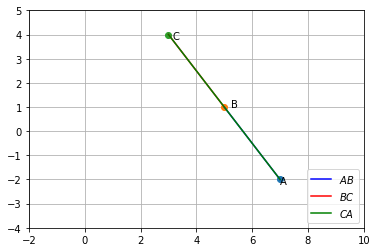
\includegraphics[width=\columnwidth]{q1a.png}
\caption{Plot of the line}
\end{figure}



\item Let $\Vec{A}=\myvec{8\\1}, \Vec{B}=\myvec{k \\ -4}, \Vec{C}=\myvec{2 \\ -5}$\\
The direction vectors of AB and AC are
\begin{align}
\label{eq:7}
\Vec{B} - \Vec{A} ={}& \myvec{k-8\\-5}\\
\label{eq:8}
\Vec{C} - \Vec{A} ={}& \myvec{-6 \\ -6}
\end{align}
\begin{align}
\label{eq:9}
\Vec{M} =\myvec{\Vec{B}-\Vec{A} & \Vec{C}-\Vec{A}}^\top
\end{align}
Substituting \eqref{eq:7} and \eqref{eq:8} in \eqref{eq:9}, we get
\begin{align}
\label{eq:10}
\Vec{M}={}&\myvec{k-8 & -5 \\ -6 & -6}
\end{align}
We know that if $rank\brak{\Vec{M}}=1$, the points are collinear.\\
Finding the rank of the matrix in the problem,
\begin{align}
\label{eq:11}
\Vec{M} = \myvec{k-8 & -6 \\ -5 & -6} \overset{R_{2}\rightarrow 5R_{2}-6R_{1}}{\longleftrightarrow} \myvec{k-8 & -5 \\ 18-6k & 0}
\end{align}
Since $rank\brak{\Vec{M}}=1$, the number of non zero rows left after doing row operations should be equal to 1.\\
Since row 1 in \eqref{eq:11} is non zero for any value of k , elements row 2 should be equal to 0.
\begin{align}
\therefore k=3
\end{align}

\begin{figure}[!h]
\centering
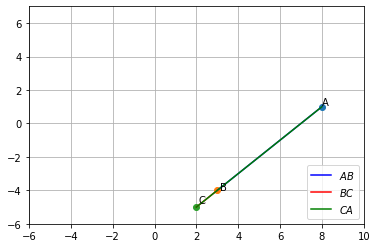
\includegraphics[width=\columnwidth]{q1b.png}
\caption{Plot of the line}
\end{figure}

\end{enumerate}
\end{document}


